% \iffalse meta-comment
%
% Copyright 1989-2005 Johannes L. Braams and any individual authors
% listed elsewhere in this file.  All rights reserved.
% 
% This file is part of the Babel system.
% --------------------------------------
% 
% It may be distributed and/or modified under the
% conditions of the LaTeX Project Public License, either version 1.3
% of this license or (at your option) any later version.
% The latest version of this license is in
%   http://www.latex-project.org/lppl.txt
% and version 1.3 or later is part of all distributions of LaTeX
% version 2003/12/01 or later.
% 
% This work has the LPPL maintenance status "maintained".
% 
% The Current Maintainers of this work are Miquel Ortega and Orestes Mas.
% 
% The list of derived (unpacked) files belonging to the distribution
% and covered by LPPL is defined by the unpacking scripts (with
% extension .ins) which are part of the distribution.
% \fi
% ^^A\CheckSum{517} TODO: update checksum when distributing. Also check version
% ^^A numbering for changes
%
% \iffalse
%    Tell the \LaTeX\ system who we are and write an entry on the
%    transcript.
%<*dtx>
\ProvidesFile{catalan.dtx}
%</dtx>
%<code>\ProvidesLanguage{catalan}
%\fi
%\ProvidesFile{catalan.dtx}
        [2020/11/01 v3.0 Catalan support from the babel system]
%\iffalse
%% File `catalan.dtx'
%
%% Catalan Language Definition File
%% Copyright (C) 1991 - 2005
%%           by Gon\c{c}al Badenes <goncal (at) badenes.cat>
%%              Johannes Braams, TeXniek
%% Copyright (C) 2020 - 2021
%%           by Miquel Ortega <miquel (dot) ortega9 (at) gmail (dot) com>
%%              Orestes Mas <orestes (dot) mas (at) upc (dot) edu>
%
%% Please report errors to: Miquel Ortega <miquel (dot) ortega9 (at) gmail (dot) com>
%%
%    This file is part of the babel system, it provides the source
%    code for the Catalan language definition file.
%    This file was developped out of spanish.sty and suggestions by
%    Gon\c{c}al Badenes <goncal (at) badenes (dot) cat> and J"org Knappen
%    <knappen (at) vkpmzd.kph.uni-mainz.de>.
%
%    The file spanish.sty was written by Julio Sanchez,
%    (jsanchez@gmv.es) The code for the catalan language has been
%    removed and now is in this file.
%<*filedriver>
\documentclass[a4paper,10pt]{ltxdoc}

% General document setup
\usepackage[left=45mm,right=40mm,top=30mm,bottom=30mm]{geometry}
\usepackage[english,catalan]{babel}

% Page setup
\setlength{\parindent}{0em}
\setlength{\parskip}{3pt}
\addtolength{\oddsidemargin}{-4pc}
\addtolength{\textwidth}{7pc}

% Font setup
\usepackage{iftex}
\ifPDFTeX
    \usepackage[utf8]{inputenc}  % Loaded by default
    \usepackage[T1]{fontenc}
    % Fonts
    \usepackage{libertinus}
    \usepackage{tipa}
    % Fake geminated L and l
    \DeclareUnicodeCharacter{013F}{L\hspace{-2pt}\raisebox{0.8pt}{\textperiodcentered}}
    \DeclareUnicodeCharacter{0140}{l\hspace{-1pt}\raisebox{0.8pt}{\textperiodcentered}\hspace{-1pt}}
\else
    % Fonts (must be installed to produce the documentation)
    \usepackage{fontspec}
    \setmainfont{Libertinus Serif}
    \setsansfont[Scale=MatchLowercase]{Libertinus Sans}
    \setmonofont[Scale=MatchLowercase]{Libertinus Mono}
\fi
\usepackage[expansion=true,protrusion=true]{microtype}
% Redefinition of the macro that prints the macro names into the left margin
\def\PrintMacroName#1{%
  \strut\MacroFont\color{DodgerBlue}\normalsize\string#1}
\def\ColorArg{\color{DodgerBlue}}

% Utilities
\usepackage[numbered]{hypdoc}  % Add hyperlink features to doc package
\PageIndex                     % Start collecting index info from macros
\RecordChanges                 % Start collecting changelog info from macros
\CodelineIndex                 % Controls if Index links are to page No. (default) or code line No.
\usepackage{graphicx}
\graphicspath{{./}{images/}}
\usepackage{amsmath}
\usepackage{booktabs}
\usepackage{placeins}
\usepackage[svgnames]{xcolor}
\usepackage{tcolorbox}
\usepackage{multirow}
\usepackage{hyperref}
\hypersetup{
  unicode=true,
	colorlinks,
	linkcolor=red,
}

% Additional logos
\usepackage{metalogo}

% Custom commands
\newcommand*\babel{\texttt{Babel}}
\newcommand*\babelcat{\texttt{babel-catalan}}
\newcommand*\Lopt[1]{\textsf{#1}}
\newcommand*\file[1]{\texttt{#1}}

% Version Info
\def\filename{catalan.dtx}
\def\filedate{\today}
\def\fileversion{3.0}

\begin{document}
  \title{Estil \textsf{catalan} per al sistema Babel\footnote{Aquest
      paquet és actualment a la versió \fileversion{} amb data del primer d'octubre
      de 2020. La present còpia del manual fou generada el~\filedate.}}
  \author{%
    Miquel Ortega\footnote{Mantenidor principal, 2020 en endavant.} \and
    Orestes Mas\footnote{Mantenidor, 2020 en endavant.} \and
    Gonçal Badenes\footnote{Autor original del paquet i mantenidor des de 1991.}%
  }
  \date{\today}
  \maketitle

  \babelcat{} és un paquet opcional que proporciona suport a l'escriptura en llengua catalana a través del sistema \babel. Està dissenyat per funcionar correctament amb els motors pdf\TeX, \XeTeX{} i Lua\TeX. Suporta els formats \texttt{Plain} i \LaTeX.

  El present document conté la guia d'ús de \babelcat: com s'ha d'emprar, quines \textit{macros} i acceleradors posa a disposició de l'usuari, el codi font del paquet i un històric de canvis. El
  document ha estat generat a partir del fitxer \file{catalan.dtx}.

  \tableofcontents

  \clearpage
  
\part{Documentació en català}

  \section{Càrrega del paquet}
    Per tal d'activar el suport al català amb \babel, especifiqueu l'opció \textbf{catalan}, 
    ja sia com a opció global o bé com a opció del paquet \babel. Pareu esment en que és la
    \textit{darrera} opció de llengua la que determina la llengua del document, per exemple:

    \verb|      \usepackage[catalan,english]{babel}|

    activa el suport al català en un document en anglès, mentre que

    \verb|      \usepackage[english,catalan]{babel}|

    estableix el català com a llengua principal del document, amb l'anglès com a llengua 
    auxiliar.

  \section{Introducció de text en català}
    \subsection{Caràcters accentuats i símbols -- mètode clàssic (actualment obsolet)}
      El programa \TeX{} original (1978-1982) reconeixia únicament els caràcters ASCII de 7 bits, per la qual cosa no era capaç de processar documents que continguessin caràcters accentuats i altres símbols. Tanmateix, aquest fet no resultava un problema per textos escrits en anglès excepte en les comptades ocasions en què calia fer ús d'aquests símbols, principalment a l'hora d'escriure noms i mots estrangers. Per aquest motiu, tant el \TeX{} com el \LaTeX{} disposen de seqüències especials per tal d'introduir els caràcters accentuats emprant únicament caràcters ASCII. Per exemple, per tal d'introduir la frase:

      \begin{center}
      \textit{Açò és un llaüt menorquí de bambú fet a mà i beneït amb cafè del flascó}
      \end{center}
      
      en \TeX/\LaTeX{} calia introduir:
      
      \begin{verbatim}
          A\c{c}\`o \'es un lla\"ut menorqu\'{\i} de bamb\'u fet a m\`a
          i bene\"{\i}t amb caf\`e del flasc\'o\end{verbatim}
      
      El paquet \babelcat{} fa les coses una mica més simples i ràpides en aquest context, definint certs caràcters com a «actius», cosa que ens estalvia d'escriure les barres invertides i claudàtors, de manera que per reproduir el text anterior només caldria escriure:
   
      \begin{verbatim}
          A"c`o 'es un lla"ut menorqu'i de bamb'u fet a m`a 
          i bene"it amb caf`e del flasc'o\end{verbatim}

      La taula \ref{tbl:acceleradors} llista les combinacions que cal emprar per accedir a aquests caràcters accentuats, així com també als caràcters de la ela geminada, guillemets i altres símbols\footnote{Pareu esment en el fet que, quan l'apòstrof és actiu, cal tenir cura d'introduir els mots apostrofats de manera que no es puguin confondre amb accents. Així, cal escriure \verb|l'\{\}estri| en lloc de \verb|l'estri|.}.

      Evidentment, introduir d'aquesta Manera els caràcters catalans especials o accentuats resulta força enutjós. Per això aquesta metodologia va caure ràpidament en desús a partir de 1990 amb l'aparició de la versió 3 de \TeX{} (\TeX90) i diverses variants capaces de treballar amb codificacions de 8 bits així com, més endavant, \XeTeX{} i {\LuaTeX{}} que accepten de forma nativa un fitxer d'entrada codificat en UTF-8. Actualment, per tant, és possible d'escriure directament els caràcters esmentats tal i com es comenta a la secció \ref{sec:moderntyping}. Tot i que de moment el paquet \babelcat{} manté la definició dels acceleradors tradicionals per qüestions de compatibilitat, aquests es consideren obsolets i podrien desaparèixer en versions futures, per la qual cosa es recomana intensament l'ús de la codificació UTF-8 i motors \TeX{} de 8 bits a l'hora de generar i processar documents nous.
      
      \clearpage

      \begin{table}[ht]
        \centering
        \caption{"<Acceleradors"> definits al paquet \babelcat}\label{tbl:acceleradors}
        \smallskip
        \begin{tabular}{ccp{7.5cm}}
          \toprule
          Per obtenir & Escriviu & Comentari\\
          \midrule
            à, è, é, í, ò, ó, ú  &  |`a|, |`e|, |'e|, |'i|, |`o|, |'o|, |'u|  &  \multirow{2}{=}{Accents greus i aguts. Per tal que aquests acceleradors funcionin, cal invocar el \textit{Babel} amb les opcions \texttt{activegrave} i \texttt{activeacute}.}\\
            À, È, É, Í, Ò, Ò, Ú  &  |`A|, |`E|, |'E|, |'I|, |`O|, |'O|, |'U| & \\
              &  &  \\
            ï, ü, ç, Ï, Ü, Ç  &  |"i|, |"u|, |"c|, |"I|, |"U|, |"C| & Dièresi i ce trencada.\\
          \midrule
            \lgem  &  |"l|, |\lgem|, |\l.l|, |·l|\footnotemark & \multirow{2}{=}{Ela geminada. Aquest dígraf es discuteix
              en profunditat a la secció \ref{sec:elageminada}.}\\
            \Lgem  &  |"L|, |\Lgem|, |\L.L|, |·L|\footnotemark[\value{footnote}] & \\
          \midrule
            "<, ">  &  |"<|, |">| & Cometes baixes o "<guillemets">, tradicionals en la tipografia catalana.\\
          \bottomrule
        \end{tabular}
      \end{table}
      \footnotetext{Només en motors Unicode}
   
  \subsection{Caràcters accentuats i símbols -- mètode modern}\label{sec:moderntyping}
    Avui en dia els principals sistemes operatius usen internament l'estàndard \textit{Unicode} i és possible d'introduir directament pel teclat els caràcters de la taula \ref{tbl:acceleradors}, amb l'excepció probable de la ela geminada, que no té un codi específic associat (vegeu la secció \ref{sec:elageminada}). Això permet d'incorporar aquests caràcters directament als fitxers d'entrada del \TeX, però caldrà indicar-li quina codificació s'ha emprat en desar-los.

    El procediment per aconseguir-ho depèn del motor \TeX{} utilitzat:
    \begin{enumerate}
      \item Si compileu els vostres documents amb \LaTeX/pdf\LaTeX, podeu  emprar el paquet \texttt{inputenc} al preàmbul per tal de poder introduir els caràcters accentuats. Com que molt probablement el vostre sistema operatiu treballarà en codificació UTF-8, haureu d'especificar-la en invocar \texttt{inputenc}:
      \begin{center}
        |\usepackage[utf8]{inputenc}|
      \end{center}
      
      \item Si esteu en un sistema UTF-8 i empreu \XeLaTeX{} o \LuaLaTeX{} per compilar els documents no caldrà que feu res més, atès que aquests motors treballen amb codificació UTF-8 de forma nativa. En el cas --rar-- que tingueu el document d'entrada en una codificació diferent a UTF-8 caldrà indicar quina al motor corresponent. En \LuaLaTeX{}, per exemple, això es fa invocant el paquet \texttt{luainputenc} de forma semblant a l'ús d'\texttt{inputenc} comentat al punt anterior (consulteu, però, la documentació).
    \end{enumerate}

  \subsection{Altres definicions del paquet \babelcat}
    Per tal de facilitar l'escriptura de documents, el paquet \babelcat{} defineix algunes ordres addicionals, que es troben llistades a la taula \ref{tbl:altres}.
    \begin{table}[ht]
      \centering
      \caption{Altres ordres definides al paquet \babelcat}\label{tbl:altres}
      \smallskip
      \begin{tabular}{lp{7.5cm}}
        \toprule
          Ordre & Efecte \\
        \midrule
          |"-|  & Guionet explícit, que permet el trencament a la resta del mot. \\
          \verb#"|# & Desactiva la lligadura a la posició actual. \\
          |\up| & Macro que ajuda a introduir caràcters de tipus ordinals amb lletres volades, com ara 1.\up{r}, 2.\up{es}, 9.\up{a}, 8.\up{ns}. Demana un argument.\\
        \bottomrule
      \end{tabular}
    \end{table}

  \subsection{La "<ela geminada">}\label{sec:elageminada}
  \subsubsection{Consideracions tipogràfiques}
    La ela geminada fou introduïda l'any 1913 per les \textit{Normes Ortogràfiques} de l'IEC per tal de representar en la llengua escrita el so de la ela doble o ela prolongada, atès que el dígraf «\textit{ll}», que era la manera tradicional de representar-lo en català antic i en llatí, havia passat progressivament a emprar-se per escriure el fonema lateral palatal \ifPDFTeX\textipa{/L/}\else/ʎ/\fi, de manera que calgué cercar una manera de diferenciar aquests
    dos sons a la llengua escrita per tal d'evitar confusions.
    
    Així, es convingué d'escriure la ela prolongada «intercalant un punt alçat entre dues \textit{l}». Segons Pompeu Fabra, les dues l que representen una ela geminada han d'anar ben juntes, gairebé tant com les dues eles que componen la ll. Això creà un símbol d'ús exclusiu en el català escrit cosa que, unida a d'altres factors, féu que l'adaptació d'aquest símbol a les noves tecnologies fos confusa i desigual, amb conflictes associats que van molt més enllà de les qüestions estètica i tipogràfica: des de disfuncions d’indexació i cerca, a problemes d’identificació que poden ser causa de processos legals.
    
  \subsubsection{Composició de la ela geminada amb el teclat de l'ordinador}
    Avui en dia la pràctica totalitat dels sistemes operatius empren internament la codificació de caràcters \textit{Unicode}. Para\l.lelament, qualsevol teclat adaptat a la llengua catalana inclourà una manera simple d'accedir al caràcter del «punt volat» (·), per la qual cosa la manera correcta d'introduir la ela geminada als nostres documents és emprant la seqüència de tres caràcters%
    \footnote{En un teclat QWERTY espanyol caldrà polsar quatre tecles: «L», («Majúscules» + «3») i «L»}
    
    IMPORTANT: Atès que l'estàndard Unicode defineix defineix una «mitja ela geminada» consistent en una ela seguida d'un punt volat (caràcters U+0139 i U+0140), temps enrere es va proposar d'introduir l'ela geminada usant aquests caràcters seguits per una ela normal: Ŀ + L = ĿL, ŀ + l = ŀl. Aquesta solució, tot i que produeix uns resultats estèticament plaents, avui en dia està \textbf{totalment desaconsellada} atès que provoca més problemes que no en resol.
    
  \subsubsection{La ela geminada en \LaTeX}
    Quan componem la ela geminada amb la seqüència «L» + «·» + «L», la majoria de tipus de lletra produeixen una ela geminada amb un espaiat excessiu entre les dues eles. Per tal de mitigar el problema, \babelcat{} ajusta l'interlletrat al voltant del punt volat. Això s'assoleix aplicant diferents estratègies segons el context:
    
   \begin{itemize}
     \item Quan el \babelcat{} s'executa en un motor Unicode, com ara \XeTeX{} o \LuaTeX, defineix les dreceres «|·|l» i «|·|L», les quals produeixen un punt volat amb l'interlletrat ajustat, seguit de la ela corresponent.
       
     \item Quan el \babelcat{} s'executa en un motor que no treballa en Unicode, com ara pdf\TeX{}, la tècnica anterior no funciona ja que el motor no treballa internament amb el punt volat com a caràcter i, en conseqüència, no es pot definir el punt volat com a caràcter «actiu» i la drecera anterior no es pot implementar. Tanmateix, si l'usuari utilitza el \LaTeX, el paquet redefineix l'objecte LICR (\LaTeX{} Internal Character Representation) anomenat \verb|\textperiodcentered| per tal d'ajustar l'interlletrat del punt volat.
   \end{itemize}
   En el cas que l'ajustament de l'interlletrat no funcioni de manera automàtica (per exemple si utilitzem el \TeX{} simple), i en interès de la retrocompatibilitat, el \babelcat{} ofereix les ordres \verb.\lgem., \verb.\Lgem., \verb|\l.l| i \verb|\L.L|, tal com s'ha especificat a la
   taula \ref{tbl:acceleradors}.

    \begin{table}[ht]
      \centering
      \caption{Aspecte de la ela geminada impresa en diversos tipus de lletra lliures usant el paquet \babelcat{} sota un motor \LuaTeX. La columna ressaltada en color correspon al mètode \textbf{desaconsellat} d'introduir la ela geminada, emprant el caràcter \textit{Unicode} «Latin Small (Capital) Letter L with Middle Dot», U+0140 (U+0139).}\label{tbl:lgem-luatex}
      \vspace{5pt}
      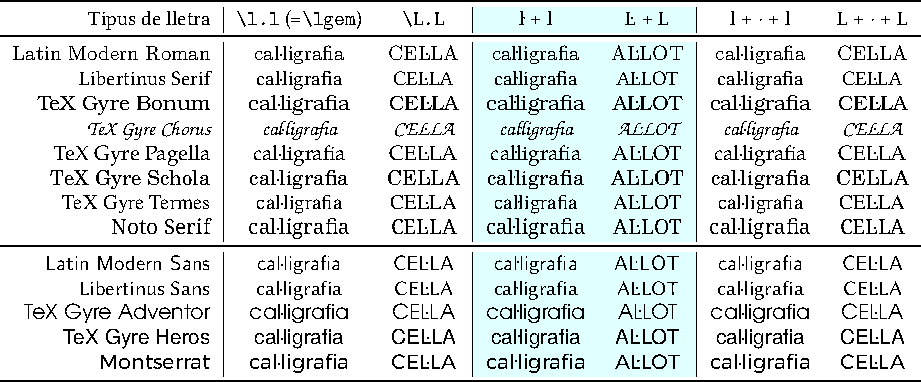
\includegraphics{lgem-luatex.pdf}
    \end{table}
    
    \begin{table}[ht]
      \centering
      \caption{Aspecte de la ela geminada impresa en diversos tipus de lletra lliures usant el paquet \babelcat{} sota un motor pdf\TeX. Noteu que amb aquest motor el mètode recomanat (\foreignlanguage{english}{l + · + l}) produeix un espaiat massa gran, que esdevé clarament erroni en el tipus \textit{Latin Modern}.}\label{tbl:lgem-pdftex}
      \vspace{5pt}
      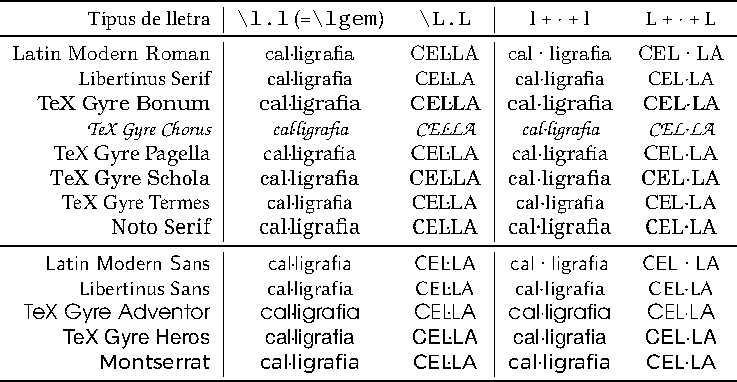
\includegraphics{lgem-pdftex.pdf}
    \end{table}

    Les taules \ref{tbl:lgem-luatex} i \ref{tbl:lgem-pdftex} ofereixen una visió més completa dels resultats que s'obtenen emprant els mètodes descrits. La primera d'elles (taula \ref{tbl:lgem-luatex}) mostra les diferents eles geminades minúscules i majúscules que s'obtenen compilant un document \LaTeX{} amb un motor Unicode (\LuaTeX{} en aquest cas) i utilitzant diversos tipus de lletra de lliure disposició. S'observa que les macros \texttt{\textbackslash lgem}, \texttt{\textbackslash l.l} i la seqüència «L» + «·» + «L» produeixen resultats idèntics.
    
    A la segona taula es mostren els mateixos resultats però en aquest cas compilant el document amb un motor no-Unicode com el pdf\LaTeX. Podem veure com en aquest cas l'espaiat entre els caràcters que componen la ela geminada és excessiu en general, i en alguns tipus de lletra concrets com ara la Latin Modern és del tot inadmissible.
 
 \FloatBarrier
 \section{Traduccions}

 \subsection{Noms de capçaleres}
   El \LaTeX{} i els seus paquets auxiliars defineixen un conjunt de noms anglesos per les
   capçaleres més habituals com ara \textit{Chapter}, \textit{Section}, \textit{Table of Contents}, 
   etcètera. El paquet \babelcat{} redefineix les macros que els generen de manera que 
   el sol fet de carregar-lo al preàmbul farà que totes aquestes capçaleres apareguin
   traduïdes al català\footnote{Si com a usuari detecteu alguna capçalera no traduïda, informeu-ne els mantenidors de \babelcat{} per tal d'incorporar la traducció en versions futures del paquet.}.

   La taula \ref{tbl:noms-capcaleres} mostra les traduccions definides a la versió actual del paquet.

   \begin{table}[ht]
     \centering
     \caption{Traduccions de capçaleres definides a \babelcat}%
     \label{tbl:noms-capcaleres}
     \smallskip
     \begin{tabular}{cll}%
       \toprule
         Definit a  &  Nom de macro           & Traducció\\%
       \midrule
         babel      &  |\prefacename|         & Pròleg\\%
         latex      &  |\refname|             & Referències\\%
         latex      &  |\abstractname|        & Resum\\%
         latex      &  |\bibname|             & Bibliografia\\%
         latex      &  |\chaptername|         & Capítol\\%
         latex      &  |\appendixname|        & Apèndix\\%
         appendix   &  |\appendixpagename|    & Apèndixs\\%
         appendix   &  |\appendixtocname|     & Apèndixs\\%
         latex      &  |\contentsname|        & Índex\\%
         latex      &  |\listfigurename|      & Índex de figures\\%
         latex      &  |\listtablename|       & Índex de taules\\%
         latex      &  |\indexname|           & Índex alfabètic\\%
         latex      &  |\figurename|          & Figura\\%
         latex      &  |\tablename|           & Taula\\%
         latex      &  |\partname|            & Part\\%
         latex      &  |\enclname|            & Adjunt\\%
         latex      &  |\ccname|              & Còpies a\\%
         latex      &  |\headtoname|          & A\\%
         latex      &  |\pagename|            & Pàgina\\%
    amscls, memoir  &  |\seename|             & Vegeu\\%
    amscls, memoir  &  |\alsoname|            & Vegeu també\\%
         amscls     &  |\proofname|           & Demostració\\%
         latex      &  |\glossaryname|        & Glossari\\%
     \bottomrule
     \end{tabular}
   \end{table}


 \subsection{Catalanitzacions en mode matemàtic}
   Per defecte, el paquet \babelcat{} defineix les versions accentuades dels operadors matemàtics
   llistats a la taula \ref{tbl:operadors}. Atès, però, que les normes d'estil de l'IEC
   recomanen d'emprar les versions sense accent, el comportament descrit es pot desactivar
   i tornar a activar amb les ordres \verb.\nocatalanoperators. i \verb.\catalanoperators.,
   respectivament.
   \begin{table}[ht]
     \centering
     \caption{Operadors matemàtics redefinits pel paquet \babelcat}
     \label{tbl:operadors}
     \smallskip
     \begin{tabular}{ccc}
       \toprule
         Operador  & versió per defecte & versió amb \verb.\nocatalanoperators. \\
       \midrule
         \verb.\mod. & $\mod$ & $\nocatalanoperators \mod$ \\
         \verb.\pmod. & $\pmod$ & $\nocatalanoperators \pmod$ \\
         \verb.\bmod. & $\bmod$ & $\nocatalanoperators \bmod$ \\
         \verb.\lim. & $\lim$ & $\nocatalanoperators \lim$ \\
         \verb.\liminf. & $\liminf$ & $\nocatalanoperators \liminf$ \\
         \verb.\limsup. & $\limsup$ & $\nocatalanoperators \limsup$ \\
         \verb.\max. & $\max$ & $\nocatalanoperators \max$ \\
         \verb.\min. & $\min$ & $\nocatalanoperators \min$ \\
         \verb.\inf. & $\inf$ & $\nocatalanoperators \inf$ \\
       \bottomrule
     \end{tabular}
   \end{table}
    
  
%%%%%%%%%%%%%%%%%%%%%%%%%%%%%%%%%%%%%%%%%%%%%%%%%%%%%%%%%%%%%%%%%%%%%%%%%%%%%%%%%%%%%%%%%%%%%%%%%%%%
%%%%%%%%%%%%%%%%%%%%%%%%%%%%%%%%%%%%%%%%%%%%%%%%%%%%%%%%%%%%%%%%%%%%%%%%%%%%%%%%%%%%%%%%%%%%%%%%%%%%
%%%%%%%%%%%%%%%%%%%%%%%%%%%%%%%%%%%%%%%%%%%%%%%%%%%%%%%%%%%%%%%%%%%%%%%%%%%%%%%%%%%%%%%%%%%%%%%%%%%%

 \clearpage

\begin{otherlanguage}{english}
\part{English Summary}

 \section{The Catalan language}
   The file \file{\filename}\footnote{The file described in this
   section has version number \fileversion{} and was last revised on
   \filedate.}  defines all language-specific macros for the
   Catalan language.

 \subsection{Translations}

 \subsubsection{Caption names}
   Catalan caption names as defined in \babelcat{} can be seen in
   Table~\ref{tab:catalan-caption-names}. They can be easily
   customised using Babel 3.9 syntax
   |\renewcommand\catalanproofname{Prova}|. The older syntax
   |\addto\captionscatalan{\renewcommand\proofname{Prova}}| still
   works.

   \begin{table}[htb]
     \centering
     \begin{tabular}{ll}%
       |\prefacename|       & Pr\`oleg\\%
       |\refname|           & Refer\`encies\\%
       |\abstractname|      & Resum\\%
       |\bibname|           & Bibliografia\\%
       |\chaptername|       & Cap\'{\i}tol\\%
       |\appendixname|      & Ap\`endix\\%
       |\appendixpagename|  & Ap\`endixs\\%
       |\appendixtocname|   & Ap\`endixs\\%
       |\contentsname|      & \'Index\\%
       |\listfigurename|    & \'Index de figures\\%
       |\listtablename|     & \'Index de taules\\%
       |\indexname|         & \'Index alfab\`etic\\%
       |\figurename|        & Figura\\%
       |\tablename|         & Taula\\%
       |\partname|          & Part\\%
       |\enclname|          & Adjunt\\%
       |\ccname|            & C\`opies a\\%
       |\headtoname|     	  & A\\%
       |\pagename|          & P\`agina\\%
       |\seename|           & Vegeu\\%
       |\alsoname|          & Vegeu tamb\'e\\%
       |\proofname|         & Demostraci\'o\\%
       |\glossaryname|      & Glossari\\%
     \end{tabular}
     \caption{Caption names as defined in \babelcat{}}%
     \label{tab:catalan-caption-names}
   \end{table}
 \subsection{Commands}
   The commands specified in Table \ref{tab:catalan-macros} are provided by
   \babelcat{} to ease typesetting.
   \begin{table}[htb]
     \centering
     \begin{tabular}{lp{8cm}}%
     |\-| & like the usual |\-|, but allowing hyphenation
              in the rest of the word. \\
     |\l.l|   & geminated-l digraph (similar to
              l$\cdot$l). |\L.L| produces the uppercase version.\\
     |\lgem|  & geminated-l digraph (similar to
              l$\cdot$l). |\Lgem| produces the uppercase version.\\
     |\up| & Macro to help typing raised ordinals, like {1\raise
              1ex\hbox{\small er}}. Takes one argument.\\
     \end{tabular}
     \caption{Commands provided by \babelcat{}}%
     \label{tab:catalan-macros}
   \end{table}

 \subsection{Shorthands}

   \babelcat{} also provides a set of shorthands to ease typing
   accents and other special characters. Note that using \emph{utf8}
   input encoding one can type the characters directly, and that
   this is enabled by default since \texttt{TexLive 2018}.

   The double quote character (|"|) is made active by default. In
   Table~\ref{tab:catalan-quote-def} an overview is given of the new
   meanings of |"|. In unicode capable engines (\XeTeX{},
   \LuaTeX{}), the interpunct character (·) is also made active to
   improve the spacing of the geminated l. See section
   \ref{sec:geminated_l_english}.

   Additionally, the user can explicitly activate the acute accent
   or apostrophe (|'|) and/or the grave accent (|`|) characters by
   using the \Lopt{activeacute} and \Lopt{activegrave} options. In
   that case, the definitions shown in
   Table~\ref{tab:catalan-quote-opt} also become
   available\footnote{Please note that if the acute accent character
   is active, it is necessary to take special care of coding
   apostrophes in a way which cannot be confounded with accents.
   Therefore, it is necessary to type \texttt{l'\{\}estri} instead
   of \texttt{l'estri}.}. These active accent characters behave
   according to their original definitions if not followed by one of
   the characters indicated in the aforementioned table.

   \begin{table}[htb]
    \centering
    \begin{tabular}{lp{8cm}}
     |"i| & i with diaeresis, allowing hyphenation
            in the rest of the word. Valid for the following vowels:
              i, u (both lowercase and uppercase).\\
     |"c| & c-cedilla (\c{c}). Valid for both uppercase and
              lowercase c.\\
     |"l| & geminated-l digraph (similar to
              l$\cdot$l). Valid for both uppercase and lowercase l.\\
     |"<| & French left double quotes (similar to $<<$).\\
     |">| & French right double quotes (similar to $>>$).\\
     |"-| & explicit hyphen sign, allowing hyphenation
              in the rest of the word.\\
     \verb="|= & disable ligature at this position.\\
     |·|l & only in unicode capable engines. See Section
     \ref{sec:geminated_l_english}.\\
     |·|L & only in unicode capable engines. See Section
     \ref{sec:geminated_l_english}.
    \end{tabular}
    \caption{Shorthands provided by \babelcat{}}
    \label{tab:catalan-quote-def}
   \end{table}

   \begin{table}[htb]
    \centering
    \begin{tabular}{lp{8cm}}
     |'e| & acute accented e, allowing hyphenation
            in the rest of the word. Valid for the following
            vowels: e, i, o, u (both lowercase and uppercase).\\
     |`a| & grave accented a, allowing hyphenation
            in the rest of the word. Valid for the following
            vowels: a, e, o (both lowercase and uppercase).
    \end{tabular}
    \caption{Extra shorthands provided by \babelcat{}
      (activated only when using the options \Lopt{activeacute} and
      \Lopt{activegrave})}
    \label{tab:catalan-quote-opt}
   \end{table}

 \subsection{Geminated l (l·l)}
   \label{sec:geminated_l_english}
   By default, most fonts produce a geminated l with incorrect
   spacing around the interpunct (·), adding too much space between
   l and l. To mitigate this, \babelcat{} adjusts the kerning around
   the interpunct. In most cases, this should be transparent to
   the user, since it is done automatically. This is achieved with
   different strategies depending on the context:
   \begin{itemize}
       \item When \babelcat{} is loaded in a Unicode capable engine,
       it defines the shorthands |·|l and |·|L, which render an
       interpunct with adjusted kerning followed by the
       corresponding l.
       \item When \babelcat{} is loaded in an engine that does not
       work in Unicode (for example, when compiling with pdf\TeX{}),
       the engine does not work internally with |·| as a character.
       Therefore, it cannot be made active, and the previous
       solution does not work. However, if working with \LaTeX{},
       the package redefines the LICR (\LaTeX{} Internal Character
       Representation) object \verb|\textperiodcentered| to adjust
       the kerning of the interpunct.
   \end{itemize}
   In case the kerning adjusment does not work automatically (for
   example, when using plain \TeX), and for the sake of backwards
   compatibility, \babelcat{} provides the commands \verb.\lgem.,
   \verb.\Lgem., \verb|\l.l| and \verb|\L.L|, as you can see in
   table \ref{tab:catalan-macros}.

 \subsection{Operators}

   By default, \babelcat{} defines accented versions of the
   mathematical operators in Table \ref{tab:catalan-operators}. The
   behaviour can be explicitly set using either
   \verb.\nocatalanoperators. or
   \verb.\catalanoperators..
   \begin{table}[htb]
    \centering
    \begin{otherlanguage}{catalan}
      \begin{tabular}{ll}
       \verb.\mod. & $\mod$\\
       \verb.\pmod. & $\pmod$\\
       \verb.\bmod. & $\bmod$\\
       \verb.\lim. & $\lim$\\
       \verb.\liminf. & $\liminf$\\
       \verb.\limsup. & $\limsup$\\
       \verb.\max. & $\max$\\
       \verb.\min. & $\min$\\
       \verb.\inf. & $\inf$
      \end{tabular}
    \end{otherlanguage}
    \caption{Math operators redefined by \babelcat{}}
    \label{tab:catalan-operators}
   \end{table}
\end{otherlanguage}
\clearpage
\newgeometry{left=50mm,right=23mm,top=30mm,bottom=30mm}
\part{Appendices}
\DocInput{catalan.dtx}
\end{document}
%</filedriver>
%\fi
%
% \StopEventually{}
%
% \changes{catalan-2.0}{1993/07/11}{Removed code to load \file{latexhax.com}}
% \changes{catalan-2.0b}{1993/09/23}{Incorporated the changes from \file{spanish.sty}}
% \changes{catalan-2.1}{1994/02/27}{Update for \LaTeXe}
% \changes{catalan-2.1d}{1994/06/26}{Removed the use of \cs{filedate}
%    and moved identification after the loading of \file{babel.def}}
% \changes{catalan-2.2b}{1995/07/04}{Made the activation of the grave and acute accents optional}
% \changes{catalan-2.2c}{1995/07/08}{Removed the use of the tilde for catalan}
% \changes{catalan-2.2f}{1996/07/13}{Replaced \cs{undefined} with
%    \cs{@undefined} and \cs{empty} with \cs{@empty} for consistency with \LaTeX}
% \changes{catalan-2.2g}{1996/10/10}{Moved the definition of \cs{atcatcode} right to the beginning.}
% \changes{catalan-2.2k}{1999/05/05}{A wrong \cs{changes} entry made typesetting impossible}
% \changes{catalan-3.0}{2020/09/01}{New maintainers. Start rework funded by IEC.}
% \changes{catalan-3.0}{2020/09/01}{Created git repo to host collaborative development}
% \changes{catalan-3.0}{2020/10/13}{Add regression tests using \texttt{l3build}}
% \changes{catalan-3.0}{2020/12/26}{Added catalan strings used by the 'appendix' package}
% \changes{catalan-3.0}{2021/03/01}{Revamped documentation. Added section in catalan.}
%
%  \section{The code}
%    The macro |\LdfInit| takes care of preventing that this file is loaded more than once, 
%    checking the category code of the \texttt{@} sign, etc.
% \changes{catalan-2.2g}{1996/11/02}{Now use \cs{LdfInit} to perform initial checks} 
%<*code>
%    \begin{macrocode}
\LdfInit{catalan}\captionscatalan
%    \end{macrocode}
%
%    When this file is read as an option, i.e. by the |\usepackage|
%    command, \texttt{catalan} could be an `unknown' language in which
%    case we have to make it known.  So we check for the existence of
%    |\l@catalan| to see whether we have to do something here.
%
% \changes{catalan-2.1d}{1994/06/26}{Now use \cs{@nopatterns} to produce the warning}
%
%    \begin{macrocode}
\ifx\l@catalan\@undefined
  \@nopatterns{Catalan}
  \adddialect\l@catalan0
\fi

\def\cat@sdef#1{\babel@save#1\def#1}
\def\cat@sDRC#1{\babel@save#1\DeclareRobustCommand*#1}
%    \end{macrocode}
%
%  \begin{macro}{\ifcat@latex}
%  \begin{macro}{\ifcat@unicode}
% \changes{catalan-3.0}{2020/10/4}{Added a new ``if'' \cs{cat@unicode} to detect unicode engines}
%
%    We define two new ifs that are set to true if we are working with
%    LaTeX and a Unicode capable engine respectively.
%
%    \begin{macrocode}
\@ifundefined{documentclass}
  {\let\ifcat@latex\iffalse}
  {\let\ifcat@latex\iftrue}

\@ifundefined{Umathcode}
  {\let\ifcat@unicode\iffalse}
  {\let\ifcat@unicode\iftrue}
%    \end{macrocode}
%  \end{macro}
%  \end{macro}
%
%  \begin{macro}{\catalanhyphenmins}
%    This macro is used to store the correct values of the hyphenation
%    parameters |\lefthyphenmin| and |\righthyphenmin|.
% \changes{catalan-2.2n}{2001/02/19}{Set the hyphenation parameters
%    both to two as required by \texttt{cahyph.tex}}
%    \begin{macrocode}
\providehyphenmins{catalan}{\tw@\tw@}
%    \end{macrocode}
%  \end{macro}
%
%  \begin{macro}{\captionscatalan}
%    The macro |\captionscatalan| defines all strings used in the four standard 
%    documentclasses provided with \LaTeX.
% \changes{catalan-1.1}{1993/07/11}{\cs{headpagename} should be \cs{pagename}}
% \changes{catalan-2.0}{1993/07/11}{Added some names}
% \changes{catalan-2.1d}{1994/11/09}{Added a few missing translations}
% \changes{catalan-2.2b}{1995/07/03}{Added \cs{proofname} for AMS-\LaTeX}
% \changes{catalan-2.2d}{1995/07/10}{added translation of Proof}
% \changes{catalan-2.2d}{1995/11/15}{Translations revised}
% \changes{catalan-2.2m}{2000/09/19}{Added \cs{glossaryname}}
% \changes{catalan-2.2p}{2003/11/17}{Inserted translation for Glossary}
% \changes{catalan-3.0}{2020/09/23}{Use Babel 3.9 syntax for captions and dates} 
% \changes{catalan-3.0}{2020/12/26}{Added catalan strings used by the \texttt{appendix} package}
%
%    Babel changed the system it used to localize captions from its
%    version 3.9 on. The change is made to allow defining strings in
%    several encodings, as xelatex/luatex do. So we changed the
%    \captionscatalan macro to the new one.
%
%    WARNING: Users of Babel prior to version 3.9 should update their
%    \TeX\ distribution to a newer one.
%
%    \begin{macrocode}
\StartBabelCommands*{catalan}{captions}
  [unicode, fontenc=TU EU1 EU2, charset=utf8]
  \SetString{\prefacename}{Pròleg}%
  \SetString{\refname}{Referències}%
  \SetString{\abstractname}{Resum}%
  \SetString{\bibname}{Bibliografia}%
  \SetString{\chaptername}{Capítol}%
  \SetString{\appendixname}{Apèndix}%
  \SetString{\appendixpagename}{Apèndixs}%
  \SetString{\appendixtocname}{Apèndixs}%
  \SetString{\contentsname}{Índex}%
  \SetString{\listfigurename}{Índex de figures}%
  \SetString{\listtablename}{Índex de taules}%
  \SetString{\indexname}{Índex alfabètic}%
  \SetString{\figurename}{Figura}%
  \SetString{\tablename}{Taula}%
  \SetString{\partname}{Part}%
  \SetString{\enclname}{Adjunt}%
  \SetString{\ccname}{Còpies a}%
  \SetString{\headtoname}{A}%
  \SetString{\pagename}{Pàgina}%
  \SetString{\seename}{Vegeu}%
  \SetString{\alsoname}{Vegeu també}%
  \SetString{\proofname}{Demostració}%
  \SetString{\glossaryname}{Glossari}%

\StartBabelCommands*{catalan}{captions}
  \SetString{\prefacename}{Pr\`oleg}%
  \SetString{\refname}{Refer\`encies}%
  \SetString{\abstractname}{Resum}%
  \SetString{\bibname}{Bibliografia}%
  \SetString{\chaptername}{Cap\'{\i}tol}%
  \SetString{\appendixname}{Ap\`endix}%
  \SetString{\appendixpagename}{Ap\`endixs}%
  \SetString{\appendixtocname}{Ap\`endixs}%
  \SetString{\contentsname}{\'Index}%
  \SetString{\listfigurename}{\'Index de figures}%
  \SetString{\listtablename}{\'Index de taules}%
  \SetString{\indexname}{\'Index alfab\`etic}%
  \SetString{\figurename}{Figura}%
  \SetString{\tablename}{Taula}%
  \SetString{\partname}{Part}%
  \SetString{\enclname}{Adjunt}%
  \SetString{\ccname}{C\`opies a}%
  \SetString{\headtoname}{A}%
  \SetString{\pagename}{P\`agina}%
  \SetString{\seename}{Vegeu}%
  \SetString{\alsoname}{Vegeu tamb\'e}%
  \SetString{\proofname}{Demostraci\'o}%
  \SetString{\glossaryname}{Glossari}%
\EndBabelCommands
%    \end{macrocode}
% \end{macro}
%
%  \begin{macro}{\datecatalan}
%    The macro |\datecatalan| redefines the command |\today| to
%    produce Catalan dates. Months are written in
%    lowercase\footnote{This seems to be the common practice. See for
%    example: E.~Coromina, \emph{El 9 Nou: Manual de redacci\'o i
%    estil}, Ed.~Eumo, Vic, 1993}.
% \changes{catalan-2.2b}{1995/06/18}{Month names in lowercase}
% \changes{catalan-2.2i}{1997/10/01}{Use \cs{edef} to define \cs{today} to save memory}
% \changes{catalan-2.2i}{1998/03/28}{use \cs{def} instead of \cs{edef}}
% \changes{catalan-3.0}{2020/09/23}{Use Babel 3.9 syntax for captions and dates}
%
%    \begin{macrocode}
\StartBabelCommands*{catalan}{date}
      [unicode, fontenc=TU EU1 EU2, charset=utf8]
  \SetStringLoop{month#1name}{gener,febrer,març,abril,maig,juny,%
    juliol,agost,setembre,octubre,novembre,desembre}

\StartBabelCommands*{catalan}{date}
  \SetStringLoop{month#1name}{gener,febrer,mar\c{c},abril,maig,juny,%
    juliol,agost,setembre,octubre,novembre,desembre}
  \SetStringLoop{month#1prep}{de ,de ,de ,d',de ,de ,%
    de ,d',de ,d',de ,de }
  \SetString\today{\number\day~\csname month\romannumeral\month
      prep\endcsname \csname month\romannumeral\month name\endcsname
  \space de~\number\year}
\EndBabelCommands
%    \end{macrocode}
%  \end{macro}
%
% \begin{macro}{\extrascatalan}
% \changes{catalan-2.0}{1993/07/11}{Macro completely rewritten}
% \changes{catalan-2.2a}{1995/03/11}{Handling of active characters
%    completely rewritten}
%
% \begin{macro}{\noextrascatalan}
% \changes{catalan-2.0}{1993/07/11}{Macro completely rewritten}
%
%    The macro |\extrascatalan| will perform all the extra definitions
%    needed for the Catalan language.  The macro |\noextrascatalan| is
%    used to cancel the actions of |\extrascatalan|.
%
%    All extras related to math are concentrated in the macro
%    mathcatalan. The rest are simply added to extrascatalan.
%
% \changes{catalan-2.2e}{1995/11/10}{Now give the apostrophe a lowercase code}
%    To improve hyphenation we give the grave character (\texttt{'}) a
%    non-zero lower case code; when we do that \TeX\ will find more
%    breakpoints in words that contain this character in its r\^ole as
%    apostrophe. 
% \changes{catalan-3.0}{2020/10/4}{Use babel@savevariable to store the
%    lowercase code of the apostrophe, and set the unicode apostrophe
%    to have a non-zero lower case code too. Code taken essentially
%    from babel-french}
%
%    \begin{macrocode}
\def\extrascatalan{%
  \mathcatalan
  }

\def\noextrascatalan{%
  \ifx\mathcatalan\@empty\else
    \nomathcatalan
  \fi}

\addto\extrascatalan{%
  \babel@savevariable{\lccode`\'}%
  \lccode`\'=`\'
  \ifcat@unicode
    \babel@savevariable{\lccode"2019}%
    \lccode"2019="2019%
  \fi
}
%    \end{macrocode}
%
%    For Catalan, some characters are made active or are redefined. In
%    particular, the \texttt{"} character receives a new meaning; this
%    can also happen for the \texttt{'} character and the \texttt{`}
%    character when the options \Lopt{activegrave} and/or
%    \Lopt{activeacute} are specified.
%
% \changes{catalan-2.2b}{1995/07/07}{Make activating the accent characters optional}
% \changes{catalan-2.2e}{1995/08/17}{Need to split up the \cs{@ifpackagewith} statements}
% \changes{catalan-3.0}{2021/04/16}{Add interpunct (``punt volat'') as active character 
%    in unicode engines.}
%
%    \begin{macrocode}
\addto\extrascatalan{\languageshorthands{catalan}}

\initiate@active@char{"}

\addto\extrascatalan{\bbl@activate{"}}

\ifcat@unicode
  \initiate@active@char{·}
  \addto\extrascatalan{\bbl@activate{·}}
\fi
%    \end{macrocode}
%    Because the grave character is being used in constructs such as
%    |\catcode``=\active| it needs to have its original category code%''
%    when the auxiliary file is being read. Note that this file is
%    read twice, once at the beginning of the document; then there is
%    no problem; but the second time it is read at the end of the
%    document to check whether any labels changes. It's this second
%    time round that the activated grave character leads to error
%    messages.
% \changes{catalan-2.2l}{1999/11/29}{Make sure that the grave accent
%    has catcode 12 \emph{before} it is made \cs{active}}
%
%    \begin{macrocode}
\@ifpackagewith{babel}{activegrave}{%
  \AtBeginDocument{%
    \if@filesw\immediate\write\@auxout{\catcode096=12}\fi}
  \initiate@active@char{`}%
  }{}

\@ifpackagewith{babel}{activegrave}{%
  \addto\extrascatalan{\bbl@activate{`}}%
  }{}

\@ifpackagewith{babel}{activeacute}{%
  \initiate@active@char{'}%
  }{}

\@ifpackagewith{babel}{activeacute}{%
  \addto\extrascatalan{\bbl@activate{'}}%
  }{}
%    \end{macrocode}
%
%    Now make sure that the characters that have been turned into
%    shorthand characters expand to `normal' characters outside the
%    catalan environment.
% \changes{catalan-2.2l}{1999/12/16}{Don't forget to deactivate the shorthands}
%
%    \begin{macrocode}
\addto\noextrascatalan{\bbl@deactivate{"}}
\@ifpackagewith{babel}{activegrave}{%
  \addto\noextrascatalan{\bbl@deactivate{`}}}{}
\@ifpackagewith{babel}{activeacute}{%
  \addto\noextrascatalan{\bbl@deactivate{'}}}{}
\ifcat@unicode
  \addto\noextrascatalan{\bbl@deactivate{·}}
\fi
%    \end{macrocode}
%
% \changes{catalan-2.2a}{1995/03/11}{All the code for handling active
%    characters is now moved to \file{babel.def}}
%
%    Apart from the active characters some other macros get a new
%    definition. We redefine them using cat@sdef so that their original
%    meaning is restored when leaving catalan.
%
%    We provide new definitions for the accent macros when one or
%    both of the options \Lopt{activegrave} or \Lopt{activeacute}
%    were specified.
%
% \changes{catalan-2.2h}{1997/01/08}{Added some comment signs to
%    prevent unwanted spaces in the output}
% \changes{catalan-3.0}{2020/10/04}{Remove diaeresis because babel already
%    handles it. Set accents with better hyphenation even if
%    activeacute or activegrave are not set}
%
%    \begin{macrocode}
\addto\extrascatalan{%
  \cat@sdef\`{\protect\cat@grave}
  \cat@sdef\'{\protect\cat@acute}
}
%    \end{macrocode}
% \end{macro}
% \end{macro}
%
%    All the code above is necessary because we need a few extra
%    active characters. These characters are then used as indicated in
%    Tables~\ref{tab:catalan-quote-def}
%    and~\ref{tab:catalan-quote-opt}.
%
%  \begin{macro}{\cat@oldacute}
% \changes{catalan-2.1d}{1994/06/26}{Renamed from \cs{acute} as that is a \cs{mathaccent}}
%  \begin{macro}{\cat@oldgrave}
% \changes{catalan-3.0}{2020/10/04}{Renamed from \cs{textacute},
%    \cs{textgrave}, to \cs{cat@oldacute}, \cs{cat@oldgrave}.}
%
%    The original definition of |\'| is stored as |\cat@oldacute|, because
%    the definition of |\'| might not be the default plain \TeX\
%    one. For this reason we save the definition of |\'| and use
%    that in the definition of other macros. We do likewise for |\`|.
%    \begin{macrocode}
\let\cat@oldgrave\`

\let\cat@oldacute\'
%    \end{macrocode}
%  \end{macro}
%  \end{macro}
%
%  \begin{macro}{\cat@acute}
%  \begin{macro}{\cat@grave}
%    We check the encoding and if not using T1, we make the accents
%    expand but enabling hyphenation beyond the accent. If this is the
%    case, not all break positions will be found in words that contain
%    accents, but this is a limitation in \TeX. An unsolved problem
%    here is that the encoding can change at any time. The definitions
%    below are made in such a way that a change between two 256-char
%    encodings are supported, but changes between a 128-char and a
%    256-char encoding are not properly supported. We check if T1 is
%    in use. If not, we will give a warning and proceed redefining the
%    accent macros so that \TeX{} at least finds the breaks that are
%    not too close to the accent. The warning will only be printed to
%    the log file.
%
%    \begin{macrocode}
\ifx\DeclareFontShape\@undefined
  \wlog{Warning: You are using an old LaTeX}
  \wlog{Some word breaks will not be found.}
    \def\cat@acute#1{\allowhyphens\cat@oldacute{#1}\allowhyphens}
    \def\cat@grave#1{\allowhyphens\cat@oldgrave{#1}\allowhyphens}
\else
  \ifx\f@encoding\bbl@t@one
      \let\cat@acute\cat@oldacute
      \let\cat@grave\cat@oldgrave
  \else
    \wlog{Warning: You are using encoding \f@encoding\space
      instead of T1.}
    \wlog{Some word breaks will not be found.}
    \def\cat@acute#1{\allowhyphens\cat@oldacute{#1}\allowhyphens}
    \def\cat@grave#1{\allowhyphens\cat@oldgrave{#1}\allowhyphens}
  \fi
\fi
%    \end{macrocode}
%  \end{macro}
%  \end{macro}
%
% \changes{catalan-2.2a}{1995/03/14}{All the code to deal with active
%    characters is now in \file{babel.def}} 
% \changes{catalan-3.0}{2021/04/16}{Add shorthands for entering ``ela
%    geminada'' directly in unicode engines.}
%
%    Now we can define our shorthands: the diaeresis and ``ela
%    geminada'' support. We only add the interpunct as a shorthand in
%    the case of a unicode engine.
%
%    \begin{macrocode}
\declare@shorthand{catalan}{"i}{\textormath{\"i}{\ddot\imath}}
\declare@shorthand{catalan}{"l}{\lgem{}}
\declare@shorthand{catalan}{"u}{\textormath{\"u}{\ddot u}}
\declare@shorthand{catalan}{"I}{\textormath{\"I}{\ddot I}}
\declare@shorthand{catalan}{"L}{\Lgem{}}
\declare@shorthand{catalan}{"U}{\textormath{\"U}{\ddot U}}

\ifcat@unicode
  \declare@shorthand{catalan}{·l}{\cat@volat{}l}%
  \declare@shorthand{catalan}{·L}{\cat@Volat{}L}%
\fi
%    \end{macrocode}
%
%    cedille,
% \changes{catalan-2.2c}{1995/07/08}{cedile now produced by double quote shorthand}
%
%    \begin{macrocode}
\declare@shorthand{catalan}{"c}{\textormath{\c c}{^{\prime} c}}
\declare@shorthand{catalan}{"C}{\textormath{\c C}{^{\prime} C}}
%    \end{macrocode}
%
%    `french' quote characters,
% \changes{catalan-2.2c}{1995/07/08}{Added shorthands for guillemets}
% \changes{catalan-2.2i}{1997/04/03}{Removed empty groups after guillemot characters}
%
%    \begin{macrocode}
\declare@shorthand{catalan}{"<}{%
  \textormath{\guillemotleft}{\mbox{\guillemotleft}}}
\declare@shorthand{catalan}{">}{%
  \textormath{\guillemotright}{\mbox{\guillemotright}}}
%    \end{macrocode}
%
%     grave accents,
% \changes{catalan-2.2e}{1996/03/05}{Added `{}` as an extra shorthand}
%
%    \begin{macrocode}
\@ifpackagewith{babel}{activegrave}{%
  \declare@shorthand{catalan}{`a}{\textormath{\cat@grave a}{\grave a}}
  \declare@shorthand{catalan}{`e}{\textormath{\cat@grave e}{\grave e}}
  \declare@shorthand{catalan}{`o}{\textormath{\cat@grave o}{\grave o}}
  \declare@shorthand{catalan}{`A}{\textormath{\cat@grave A}{\grave A}}
  \declare@shorthand{catalan}{`E}{\textormath{\cat@grave E}{\grave E}}
  \declare@shorthand{catalan}{`O}{\textormath{\cat@grave O}{\grave O}}
  \declare@shorthand{catalan}{``}{\textquotedblleft}%''
  }{}
%    \end{macrocode}
%
%     acute accents,
% \changes{catalan-2.2b}{1995/07/03}{Changed mathmode definition of acute shorthands to expand 
%    to a single prime followed by the next character in the input}
% \changes{catalan-2.2e}{1995/09/05}{Added vertical bar as argument to active acute}
%
%    \begin{macrocode}
\@ifpackagewith{babel}{activeacute}{%
  \declare@shorthand{catalan}{'a}{\textormath{\cat@acute a}{^{\prime} a}}
  \declare@shorthand{catalan}{'e}{\textormath{\cat@acute e}{^{\prime} e}}
  \declare@shorthand{catalan}{'i}{\textormath{\cat@acute\i{}}{^{\prime} i}}
  \declare@shorthand{catalan}{'o}{\textormath{\cat@acute o}{^{\prime} o}}
  \declare@shorthand{catalan}{'u}{\textormath{\cat@acute u}{^{\prime} u}}
  \declare@shorthand{catalan}{'A}{\textormath{\cat@acute A}{^{\prime} A}}
  \declare@shorthand{catalan}{'E}{\textormath{\cat@acute E}{^{\prime} E}}
  \declare@shorthand{catalan}{'I}{\textormath{\cat@acute I}{^{\prime} I}}
  \declare@shorthand{catalan}{'O}{\textormath{\cat@acute O}{^{\prime} O}}
  \declare@shorthand{catalan}{'U}{\textormath{\cat@acute U}{^{\prime} U}}
  \declare@shorthand{catalan}{'|}{%
    \textormath{\csname normal@char\string'\endcsname}{^{\prime}}}
%    \end{macrocode}
%
%    the acute accent,
% \changes{catalan-2.2c}{1995/07/08}{Added '{}' as an extra shorthand, removed 'n as a shorthand}
%
%    \begin{macrocode}
\declare@shorthand{catalan}{''}{%
  \textormath{\textquotedblright}{\sp\bgroup\prim@s'}}
}{}
%    \end{macrocode}
%
%    and finally, some support definitions
%
%    \begin{macrocode}
\declare@shorthand{catalan}{"-}{\nobreak-\bbl@allowhyphens}
\declare@shorthand{catalan}{"|}{%
  \textormath{\nobreak\discretionary{-}{}{\kern.03em}%
              \bbl@allowhyphens}{}}
%    \end{macrocode}
%
%  \begin{macro}{\-}
%
%    All that is left now is the redefinition of |\-|. The new version
%    of |\-| should indicate an extra hyphenation position, while
%    allowing other hyphenation positions to be generated
%    automatically. The standard behaviour of \TeX\ in this respect is
%    unfortunate for Catalan but not as much as for Dutch or German,
%    where long compound words are quite normal and all one needs is a
%    means to indicate an extra hyphenation position on top of the
%    ones that \TeX\ can generate from the hyphenation patterns.
%    However, the average length of words in Catalan makes this
%    desirable and so it is kept here.
%
%    \begin{macrocode}
\addto\extrascatalan{%
  \babel@save{\-}%
  \def\-{\bbl@allowhyphens\discretionary{-}{}{}\bbl@allowhyphens}}
%    \end{macrocode}
%  \end{macro}
%
%  \begin{macro}{\cat@volat}
%  \begin{macro}{\cat@Volat}
% \changes{catalan-3.0}{2021/04/16}{Separate lgem definition from the interpunct
%    (``punt volat'') definition. Define cat@volat as the interpunct with some
%    kerning adjustments.}
%
%    The macros \verb.\cat@volat. and \verb.\cat@Volat. print the interpunct
%    with adjusted kerning. The first adjusts the kerning for the lower case
%    geminated l and the second one for the upper case one.
%
%    \begin{macrocode}
\newdimen\leftllkern \newdimen\rightllkern \newdimen\raiselldim

\def\cat@volat{%
  \leftllkern=0pt\rightllkern=0pt\raiselldim=0pt%
  \setbox0\hbox{l}\setbox1\hbox{l}\setbox2\hbox{\cat@oldvolat}%
  \advance\leftllkern by -0.5\wd2%
  \advance\rightllkern by -0.5\wd2%
  \advance\leftllkern by 0.2\wd0%
  \advance\rightllkern by 0.2\wd0%
  \bbl@allowhyphens\discretionary{-}{}%
  {\kern\leftllkern\raise\raiselldim\box2%
  \kern\rightllkern}\bbl@allowhyphens%
}

\def\cat@Volat{%
  \leftllkern=0pt\rightllkern=0pt\raiselldim=0pt%
  \setbox0\hbox{L}\setbox1\hbox{L}\setbox2\hbox{\cat@oldvolat}%
  \advance\leftllkern by -0.5\wd2%
  \advance\rightllkern by -0.5\wd2%
  \advance\leftllkern by -0.25\wd0%
  \advance\rightllkern by 0.2\wd0%
  \advance\raiselldim by 0.1\ht0%
  \bbl@allowhyphens\discretionary{-}{}%
  {\kern\leftllkern\raise\raiselldim\box2%
  \kern\rightllkern}\bbl@allowhyphens%
}
%    \end{macrocode}
%  \end{macro}
%  \end{macro}
%
% \changes{catalan-3.0}{2020/04/16}{Redefine ``\textperiodcentered'' when
%    possible to allow entering ``ela geminada'' directly in non-unicode
%    engines.}
%
%    If possible, we redefine \verb.\textperiodcentered. to adjust its
%    kerning. This way, a user can enter directly the geminated l and
%    obtain better results than the ones obtained by default. Note
%    that this solution does not cover the unicode capable engines,
%    since it only redefines the LICR. For the latter case, we also
%    define appropriate shorthands.
%
%    \begin{macrocode}
\@ifundefined{textperiodcentered}{}{
  \expandafter\let\expandafter\cat@oldvolat
  \csname ?\string\textperiodcentered \endcsname
  \DeclareTextCommand{\textperiodcentered}{?}{%
    \@ifnextchar{l}{\cat@volat{}}{%
      \@ifnextchar{L}{\cat@Volat{}}{%
      \cat@oldvolat}%
    }%
  }%
}
%    \end{macrocode}
%
%  \begin{macro}{\lgem}
%  \begin{macro}{\Lgem}
% \changes{catalan-2.2b}{1995/06/18}{Added support for typing the
%    catalan ``ela geminada'' with the macros \cs{lgem} and \cs{Lgem}}
% \changes{catalan-2.2f}{1996/09/20}{Added a check for math mode as
%    the use of \cs{lgem} and \cs{Lgem} in math mode is not sensible.}
% \changes{catalan-3.0}{2020/10/31}{Use ``\textperiodcentered'' when available to
%    produce the middle dot. This allows both searching and copy and paste, and
%    gives somewhat better results than the plain macro.}
%
%    Here we define two macros for typesetting the catalan ``ela geminada''
%    (geminated l). The sequences |\lgem| and |\Lgem| have been chosen
%    for its lowercase and uppercase representation,
%    respectively\footnote{The macro names \cs{ll} and \cs{LL} were
%    not chosen because \cs{ll} is already used in
%    mathematical mode.}. If available we use the command
%    \verb|\textperiodcentered| to output the middle dot, but we still adjust
%    its horizontal kerning, since most fonts get it wrong. If this command is
%    unavailable, we use a plain \TeX{} definition.
%
%    The code used in the plain \TeX{} definition is a combination of
%    the one proposed by Valiente and Fuster\footnote{G.~Valiente and
%    R.~Fuster, Typesetting Catalan Texts with \TeX, \emph{TUGboat}
%    \textbf{14}(3), 1993.} and the proposal\footnote{G. Valiente,
%    Modern Catalan Typographical Conventions, \emph{TUGboat}
%    \textbf{16}(3), 1995.} from Valiente presented at the \TeX\ Users
%    Group Annual Meeting in 1995. This last proposal was not fully
%    implemented due to its limitation to CM fonts.
%
%    \begin{macrocode}
\def\lgem{%
  \ifmmode
    \csname normal@char\string"\endcsname l%
  \else
    \leftllkern=0pt\rightllkern=0pt\raiselldim=0pt%
    \@ifundefined{textperiodcentered}{
      \setbox0\hbox{l}\setbox1\hbox{l\/}\setbox2\hbox{.}%
      \advance\raiselldim by \the\fontdimen5\the\font%
      \advance\raiselldim by -\ht2%
      \leftllkern=-.25\wd0%
      \advance\leftllkern by \wd1%
      \advance\leftllkern by -\wd0%
      \rightllkern=-.25\wd0%
      \advance\rightllkern by -\wd1%
      \advance\rightllkern by \wd0%
      \bbl@allowhyphens\discretionary{l-}{l}%
      {\hbox{l}\kern\leftllkern\raise\raiselldim\box2%
      \kern\rightllkern\hbox{l}}\bbl@allowhyphens%
    }{l\cat@volat{}l}%
  \fi
}

\def\Lgem{%
  \ifmmode
    \csname normal@char\string"\endcsname L%
  \else
    \leftllkern=0pt\rightllkern=0pt\raiselldim=0pt%
    \@ifundefined{textperiodcentered}{
      \setbox0\hbox{L}\setbox1\hbox{L\/}\setbox2\hbox{.}%
      \advance\raiselldim by .5\ht0%
      \advance\raiselldim by -.5\ht2%
      \leftllkern=-.125\wd0%
      \advance\leftllkern by \wd1%
      \advance\leftllkern by -\wd0%
      \rightllkern=-\wd0%
      \divide\rightllkern by 6%
      \advance\rightllkern by -\wd1%
      \advance\rightllkern by \wd0%
      \bbl@allowhyphens\discretionary{L-}{L}%
      {\hbox{L}\kern\leftllkern\raise\raiselldim\box2%
      \kern\rightllkern\hbox{L}}\bbl@allowhyphens%
    }{L\cat@Volat{}L}%
  \fi
}
%    \end{macrocode}
%  \end{macro}
%  \end{macro}
%
%  \begin{macro}{\l.l}
%  \begin{macro}{\L.L}
% \changes{catalan-2.2e}{1996/06/26}{Added redefinition of \cs{l} and
%    \cs{L}}
% \changes{catalan-2.2o}{2003/09/19}{Postpone the redefinition of
%    \cs{l} and \cs{L} until begin document to prevent overwriting by fontenc}
%
%    We define the sequences |\l.l| and |\L.L|. These are not really
%    macro's by themselves but the macros |\l| and |\L| with delimited
%    arguments. Therefore we define two macros that check if the next
%    character is a period. If not the ``polish l'' will be typeset,
%    otherwise a ``ela geminada'' will be typeset and the next two
%    tokens will be ``eaten''.
%
%    \begin{macrocode}
\AtBeginDocument{%
  \let\cat@lslash\l
  \let\cat@Lslash\L
  \DeclareRobustCommand\l{\@ifnextchar.\cat@l\cat@lslash}
  \DeclareRobustCommand\L{\@ifnextchar.\cat@L\cat@Lslash}}

\def\cat@l#1#2{\lgem}
\def\cat@L#1#2{\Lgem}
%    \end{macrocode}
%  \end{macro}
%  \end{macro}
%
%  \begin{macro}{\up}
%
%    A macro for typesetting things like 1\raise1ex\hbox{\small er} as
%    proposed by Raymond S\'{e}roul\footnote{This macro has been borrowed
%    from francais.dtx}.
% \changes{catalan-2.2b}{1995/06/18}{Added definition of macro \cs{up}, 
%    which can be used to type ordinals}
% \changes{catalan-2.2e}{1996/02/29}{Now use \cs{textsuperscript} and make \cs{up} robust}
%
%    \begin{macrocode}
\DeclareRobustCommand*{\up}[1]{\textsuperscript{#1}}
%    \end{macrocode}
%  \end{macro}
%
%   In catalan, some of the operators in math need to have accents. 
%   It's not easy to add an accent to an operator, because we must 
%   avoid using text (that is, |\mbox|) where we have no control on 
%   font and size, and at the same time we need |\i|, which is forbidden 
%   in math mode. We use |\dotlessi| to do so and add the accents to
%   the corresponding operators\footnote{This implementation has been
%   borrowed from spanish.dtx}.
% \changes{catalan-3.0}{2020/11/10}{Added accented math operators}
%
%    \begin{macrocode}
\addto\mathcatalan{\cat@sDRC\dotlessi{\cat@dotlessi}}
\let\nomathcatalan\relax

\ifcat@latex
  \def\cat@texti{\i}
  \addto\@uclclist{\dotlessi\cat@texti}
\fi

\def\cat@fetchenc{%
  \count@\escapechar \escapechar=\m@ne
    \edef\cat@a{\expandafter\string\the\textfont\mathgroup}%
    \expandafter\split@name\cat@a////\@nil
  \escapechar=\count@
  \@expandtwoargs\in@{////}{\f@size}%
  \ifin@\else
    \PackageError{catalan}{%
      Non-NFSS font name. The current math font (\cat@a)\MessageBreak
      doesn't follow the NFSS conventions. I'll use the\MessageBreak
      default \string\i\space for \string\dotlessi,
      but expect a wrong output.}%
    {Find where this font has been (re)defined, and fix it.}%
    \def\f@encoding{OT1}%
  \fi}

\ifcat@latex
  \ifx\Umathchardef\@undefined\else
    \expandafter\Umathchardef\csname cat@EU1@dotlessi\endcsname"7"1"0131\relax
    \expandafter\Umathchardef\csname cat@EU2@dotlessi\endcsname"7"1"0131\relax
    \expandafter\Umathchardef\csname cat@TU@dotlessi\endcsname"7"1"0131\relax
  \fi
  \def\cat@dotlessi{%
    \ifmmode
      {\ifnum\mathgroup=\m@ne
         \imath
       \else
         \cat@fetchenc
         \@ifundefined{cat@\f@encoding @dotlessi}%
           {\@ifundefined{\f@encoding\string\i}%
             {\edef\f@encoding{\string?}}{}%
            \expandafter\count@\the\csname\f@encoding\string\i\endcsname
            \advance\count@"7000
            \mathchar\count@}%
           {\csname cat@\f@encoding @dotlessi\endcsname}%
       \fi}%
    \else
      \i
    \fi}
\else
  \def\cat@dotlessi{\textormath{\i}{\mathchar"7010}}
\fi
%    \end{macrocode}
%
%    As math mode doesn't have accented characters, we need to
%    specifically define and add the accented characters using
%    unicode.
%
%    \begin{macrocode}
\def\cat@op@ac@base#1{\acute{\if i#1\dotlessi\else#1\fi}}
\def\cat@op@gr@base#1{\grave{\if i#1\dotlessi\else#1\fi}}

\ifx\Umathchar\@undefined\else
  \def\cat@ac@TU@e{"00E9}\def\cat@ac@TU@E{"00C9}%
  \def\cat@ac@TU@i{"00ED}\def\cat@ac@TU@I{"00CD}%
  \def\cat@ac@TU@o{"00F3}\def\cat@ac@TU@O{"00D3}%
  \def\cat@ac@TU@u{"00FA}\def\cat@ac@TU@U{"00DA}%
  \def\cat@gr@TU@a{"00E0}\def\cat@gr@TU@A{"00C0}%
  \def\cat@gr@TU@e{"00E8}\def\cat@gr@TU@E{"00C8}%
  \def\cat@gr@TU@o{"00F2}\def\cat@gr@TU@O{"00D2}%
  \def\cat@op@ac@TU#1{%
    \ifnum\mathgroup=\m@ne
      \cat@op@ac@base{#1}%
    \else
      \cat@fetchenc
      \@ifundefined{cat@op@ac@\f@encoding}%
        {\cat@op@ac@base{#1}}%
        {\@ifundefined{cat@ac@TU@#1}%
           {\cat@op@ac@base{#1}}%
           {\Umathchar"7"1\csname cat@ac@TU@#1\endcsname}}%
    \fi}%
  \def\cat@op@gr@TU#1{%
    \ifnum\mathgroup=\m@ne
      \cat@op@gr@base{#1}%
    \else
      \cat@fetchenc       
      \@ifundefined{cat@op@gr@\f@encoding}%
        {\cat@op@gr@base{#1}}%
        {\@ifundefined{cat@gr@TU@#1}%
           {\cat@op@gr@base{#1}}%
           {\Umathchar"7"1\csname cat@gr@TU@#1\endcsname}}%
    \fi}%
  \expandafter\let\csname cat@op@ac@EU1\endcsname\cat@op@ac@TU
  \expandafter\let\csname cat@op@ac@EU2\endcsname\cat@op@ac@TU
  \expandafter\let\csname cat@op@gr@EU1\endcsname\cat@op@gr@TU
  \expandafter\let\csname cat@op@gr@EU2\endcsname\cat@op@gr@TU
\fi
%    \end{macrocode}
%
% \begin{macro}{\catalanoperators}
% \begin{macro}{\nocatalanoperators}
%    The macro |\catalanoperators| enables the corresponding
%    accented operators, active by default.
%    The macro |\nocatalanoperators| is used
%    to cancel the actions of |\catalanoperators|.
%
%    \begin{macrocode}
\def\catalanoperators{%
  \@ifundefined{cat@op@ac@TU}%
    {\let\cat@op@ac\cat@op@ac@base}%
    {\let\cat@op@ac\cat@op@ac@TU}
  \@ifundefined{cat@op@gr@TU}%
    {\let\cat@op@gr\cat@op@gr@base}%
    {\let\cat@op@gr\cat@op@gr@TU}}

\def\nocatalanoperators{%
  \def\cat@op@ac##1{##1}
  \def\cat@op@gr##1{##1}}

\catalanoperators
%    \end{macrocode}
%  \end{macro}
%  \end{macro}
%
%    \begin{macrocode}
\addto\mathcatalan{\cat@operators}

\ifcat@latex\else
  \let\operator@font\rm
\fi
%    \end{macrocode}
%
%    Operators are stored in |\cat@operators|, which is
%    included in the math group. Since |\operator@font| is
%    defined in \LaTeXe{} only, we define it in the plain variant.
%
%    \begin{macrocode}
\def\cat@operators{%
  \cat@sdef\bmod{\nonscript\mskip-\medmuskip\mkern5mu
    \mathbin{\operator@font m\cat@op@gr od}\penalty900\mkern5mu
    \nonscript\mskip-\medmuskip}%
  \@ifundefined{@amsmath@err}%
    {\cat@sdef\pmod##11{\allowbreak\mkern18mu
        ({\operator@font m\cat@op@gr od}\,\,##11)}}%
    {\cat@sdef\mod##1{\allowbreak\if@display\mkern18mu
        \else\mkern12mu\fi{\operator@font m\cat@op@gr od}\,\,##1}%
      \cat@sdef\pmod##1{\pod{{\operator@font m\cat@op@gr od}%
        \mkern6mu##1}}}%
  \cat@sdef\lim{\mathop{\operator@font l\cat@op@ac im}}
  \cat@sdef\liminf{\mathop{\operator@font l\cat@op@ac im\, inf}}
  \cat@sdef\limsup{\mathop{\operator@font l\cat@op@ac im\, sup}}
  \cat@sdef\max{\mathop{\operator@font m\cat@op@gr ax}}
  \cat@sdef\inf{\mathop{\operator@font \cat@op@ac inf}}
  \cat@sdef\min{\mathop{\operator@font m\cat@op@ac in}}
  }
%    \end{macrocode}
%
%    The macro |\ldf@finish| takes care of looking for a
%    configuration file, setting the main language to be switched on
%    at |\begin{document}| and resetting the category code of
%    \texttt{@} to its original value.
% \changes{catalan-2.2g}{1996/11/02}{Now use \cs{ldf@finish} to wrap up}
%
%    \begin{macrocode}
\ldf@finish{catalan}
%    \end{macrocode}
%
% \Finale 
% \clearpage
% \PrintIndex
% \PrintChanges
%
%% \CharacterTable
%%  {Upper-case    \A\B\C\D\E\F\G\H\I\J\K\L\M\N\O\P\Q\R\S\T\U\V\W\X\Y\Z
%%   Lower-case    \a\b\c\d\e\f\g\h\i\j\k\l\m\n\o\p\q\r\s\t\u\v\w\x\y\z
%%   Digits        \0\1\2\3\4\5\6\7\8\9
%%   Exclamation   \!     Double quote  \"     Hash (number) \#
%%   Dollar        \$     Percent       \%     Ampersand     \&
%%   Acute accent  \'     Left paren    \(     Right paren   \)
%%   Asterisk      \*     Plus          \+     Comma         \,
%%   Minus         \-     Point         \.     Solidus       \/
%%   Colon         \:     Semicolon     \;     Less than     \<
%%   Equals        \=     Greater than  \>     Question mark \?
%%   Commercial at \@     Left bracket  \[     Backslash     \\
%%   Right bracket \]     Circumflex    \^     Underscore    \_
%%   Grave accent  \`     Left brace    \{     Vertical bar  \|
%%   Right brace   \}     Tilde         \~}
%%
\endinput
